


%	PACKAGES AND OTHER DOCUMENT CONFIGURATIONS

\documentclass[
	12pt, % Default font size, values between 10pt-12pt are allowed
	%letterpaper, % Uncomment for US letter paper size
	%spanish, % Uncomment for Spanish
]{style/fphw}

% Template-specific packages

\usepackage[utf8]{inputenc} % Required for inputting international characters
\usepackage[T1]{fontenc} % Output font encoding for international characters
\usepackage{mathpazo} % Use the Palatino font
\usepackage{amssymb}
\usepackage{graphicx} % Required for including images
\usepackage{booktabs} % Required for better horizontal rules in tables
\usepackage{listings} % Required for insertion of code
\usepackage{enumerate} % To modify the enumerate environment
\usepackage{epstopdf}
% \epstopdfDeclareGraphicsRule{.tif}{png}{.png}{convert #1 \OutputFile}
\AppendGraphicsExtensions{.tif}
\usepackage[ruled,vlined]{algorithm2e}
\usepackage{minted}
\usepackage[nottoc]{tocbibind}
\usepackage{caption}
\usepackage{subcaption}
\usepackage{mathtools}
\DeclarePairedDelimiter\abs{\lvert}{\rvert}%
\DeclarePairedDelimiter\norm{\lVert}{\rVert}%

% Swap the definition of \abs* and \norm*, so that \abs
% and \norm resizes the size of the brackets, and the 
% starred version does not.
\makeatletter
\let\oldabs\abs
\def\abs{\@ifstar{\oldabs}{\oldabs*}}
%
\let\oldnorm\norm
\def\norm{\@ifstar{\oldnorm}{\oldnorm*}}
\makeatother



\graphicspath{{/Users/tongyuan/Documents/Study/S6_Spring_2021/Digital_Imagine_Processing/EE326_Digital_Image_Processing_LAB/Lab6_Image_Restoration/plots}}

%----------------------------------------------------------------------------------------
%	ASSIGNMENT INFORMATION
%----------------------------------------------------------------------------------------

\title{Lab 6 Frquency Domain Filtering} % Assignment title

\author{YUAN Tong 11810818} % Student name

%\date{March 28th, 2025} % Due date

\institute{Southern University of Science and Technology \\ School of Microelectronic} % Institute or school name

\class{LAB Session I} % Course or class name

\professor{YU Yajun} % Professor or teacher in charge of the assignment

%----------------------------------------------------------------------------------------

\begin{document}
\definecolor{bg}{rgb}{0.95,0.95,0.95}
\maketitle % Output the assignment title, created automatically using the information in the custom commands above

%----------------------------------------------------------------------------------------
%	ASSIGNMENT CONTENT
%----------------------------------------------------------------------------------------

\section*{Introduction}
The objective of restoration is to improve a given image in some predefined sense. Compare with image enhancement which is largely a subjective process, image restoration is for the most part an objective process. When we apply image restoring to a degraded image, we will first construct a model about how the image was degraded and then we apply the degrade filter to the restoring filter. After that we could get the reconstructed image, however, we can't build the degrade model precisely and there may be some overlap in frequency domain after the image was degrade, so we can not always restore that image like what it used to be.

In this lab, there are three tasks will be performed.

\begin{enumerate}
	\item Apply adeptive filter to the image with high noise intensity
	\item Apply full inverse filtering, radially limited inverse filtering and Wiener filtering to a image degraded by atomsphere turbulence. Discuss how the parameters, if any, are determined, and the different effects by using the different algorithms.
	\item Restore a image degraded by motion blur and noise.
\end{enumerate}

%----------------------------------------------------------------------------------------
%	TASKS
%----------------------------------------------------------------------------------------

\newpage
\section*{Task I: Adaptive Filter for Image Denoising}

\begin{problem}
	Remove the noise from the input images Q6\_1\_1.tif, Q6\_1\_2.tif, Q6\_1\_3.tif and Q6\_1\_4.tif. Explain your observation and the method used to each of the images, and why such methods are used.

	\begin{figure}[H]
		\centering
		\begin{subfigure}[b]{.24\textwidth}
			\centering
			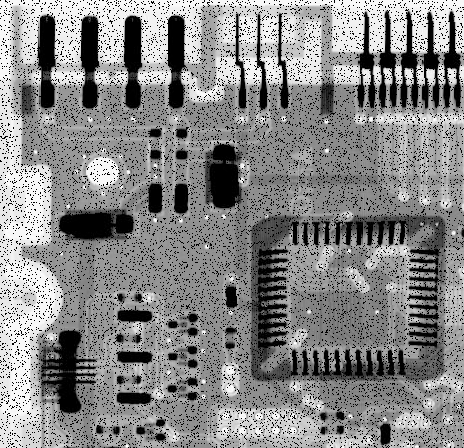
\includegraphics[width=0.9\linewidth]{Q6_1_1.png}
			\caption{Q6\_1\_1}
			\label{Q6_1_1}
		\end{subfigure}
		\hfill
		\begin{subfigure}[b]{.24\textwidth}
			\centering
			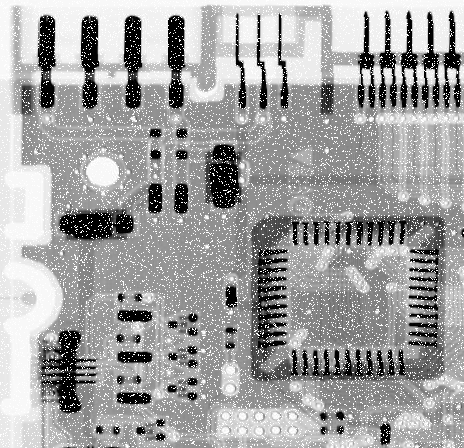
\includegraphics[width=0.9\linewidth]{Q6_1_2.png}
			\caption{Q6\_1\_2}
			\label{Q6_1_2}
		\end{subfigure}
		\hfill
		\begin{subfigure}[b]{.24\textwidth}
			\centering
			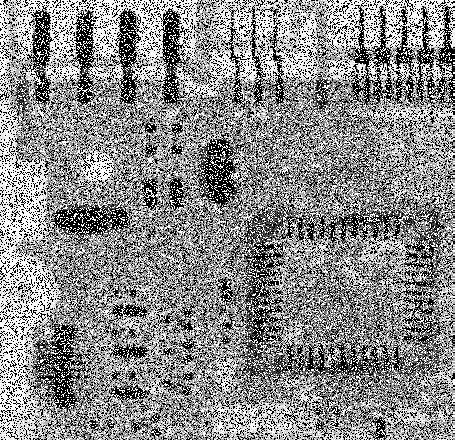
\includegraphics[width=0.9\linewidth]{Q6_1_3.png}
			\caption{Q6\_1\_3}
			\label{Q6_1_3}
		\end{subfigure}
		\hfill
		\begin{subfigure}[b]{.24\textwidth}
			\centering
			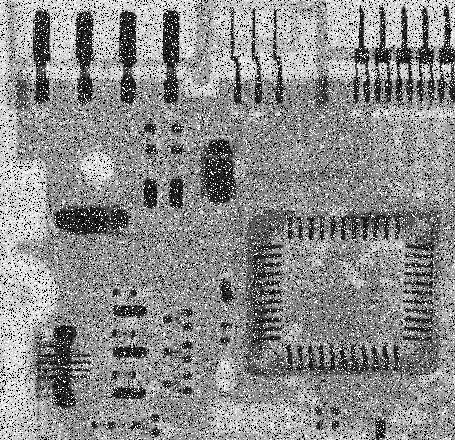
\includegraphics[width=0.9\linewidth]{Q6_1_4.png}
			\caption{Q6\_1\_4}
			\label{Q6_1_4}
		\end{subfigure}
		\caption{Task I, Figures with noise}
    	\label{Task I, Figures with noise}	
	\end{figure}
\end{problem}

\subsection*{Analysis}

	For traditional noise filter in spstial domain, the size of the filter is limited, here comes the problem: if the size of the filter is too small, for areas with hihg noise intensity, the filetr can't reduce all the noise, for example, when a apply a midtern filter to a 3X3 sqare with more than 5 pixels are noise with 255, the midterm will always be the 255, for average filter, the number of the result will be greatly affected by the noise.
	
	\textbf{To solve this problem, two differnet methods are designed.}


	\subsubsection*{Smart filter}
	The first method is called "smart filter". The filter will analysis the noise situation of the square being filtered, if the noise intensity in the square is high, some pixels in extremely high or low intensity will be removed in future operation. The procedure of the algorithms is shown below.

	\IncMargin{1em}
	\begin{algorithm}
		\DontPrintSemicolon
		\SetKwInOut{Input}{input}\SetKwInOut{Output}{output}

		\Input{The image with noise}
		\Output{The denoised image}

		\BlankLine
		\ForAll{Pixels in the given image}{
			\If{Pixels with intensity between (5, 250) is contianed in the image}{
				Find the normal pixel most close to the middle
			}
			\Else{
				Calculate the average value
			}
			Assign the value to the related pixels in the output image
		}
		\caption{Smart denoise filter}
	\end{algorithm}


	\subsubsection*{Adaptive filter}
	In this method, if the given square has high noise intensity, we will expand the size of the filter until the noise intensity in the domain fit our requirement. The procedure is shown below.

	\begin{algorithm}[H]
		\DontPrintSemicolon
		\SetKwInOut{Input}{input}\SetKwInOut{Output}{output}

		\Input{The image with noise, the initial size, the max size}
		\Output{The denoised image}

		$S_{xy}$: The domain we apply the filter \\
		$z_{min}$: The minimum intensity value in $S_{xy}$  \\
		$z_{max}$: The maximum intensity value in $S_{xy}$  \\
		$z_{med}$: median intensity value in $S_{xy}$       \\
		$z_{xy}$: intensity value at coordinates (x, y) \\
		$S_{max}$: maximum allowed size of $S_{xy}$ \\

		\BlankLine
		\ForAll{Pixels in the given image}{
			\Repeat{output is generated}{
				$A_1 = z_{med} - z_{min}$  \\
				$A_2 = z_{med} - z_{max}$  \\
				\If{$A_1 > 0$ and $A_2 < 0$}{
					$B_1 = z_{xy} - z_{min}$  \\
					$B_2 = z_{xy} - z_{max}$  \\
					\If{$B_1 > 0$ and $B_2 < 0$}{
						output $z_{xy}$ 	
					}
					\Else{
						output $z_{med}$
					}
				}
				\Else{
					Increase the size of $S_{xy}$
					\If{size < $S_max$}{
						repeat the loop
					}
					\Else{
						output $z_{med}$
					}

				}
			}
			
		}
		\caption{Smart denoise filter}
	\end{algorithm}

	\subsection*{Result}
	
	After applying both filter to the given given image, we obtain the following results

	\begin{figure}[H]
		\centering
		\begin{subfigure}[b]{.24\textwidth}
			\centering
			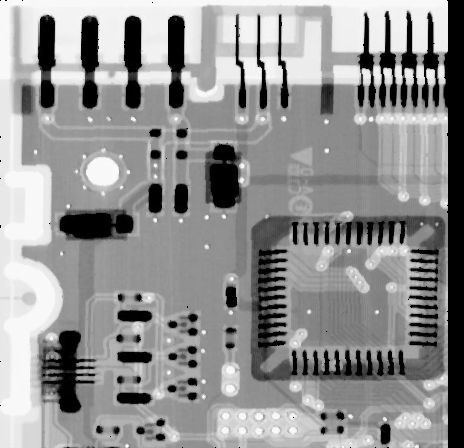
\includegraphics[width=0.9\linewidth]{Q6_1_1_denoised.png}
			\caption{Q6\_1\_1\_denoised}
			\label{Q6_1_1_denoised}
		\end{subfigure}
		\hfill
		\begin{subfigure}[b]{.24\textwidth}
			\centering
			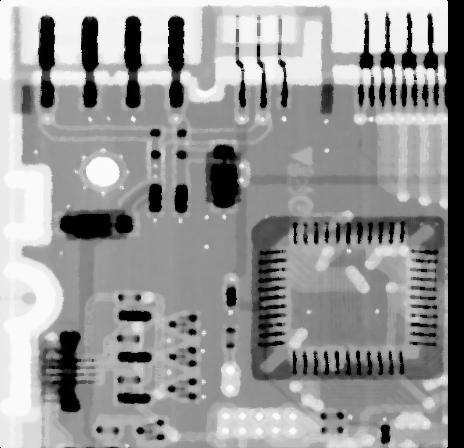
\includegraphics[width=0.9\linewidth]{Q6_1_2_denoised.png}
			\caption{Q6\_1\_2\_denoised}
			\label{Q6_1_2_denoised}
		\end{subfigure}
		\hfill
		\begin{subfigure}[b]{.24\textwidth}
			\centering
			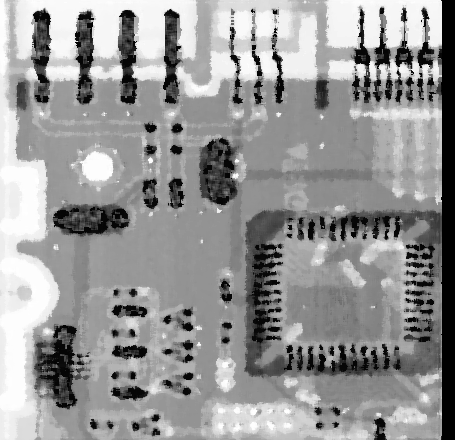
\includegraphics[width=0.9\linewidth]{Q6_1_3_denoised.png}
			\caption{Q6\_1\_3\_denoised}
			\label{Q6_1_3_denoised}
		\end{subfigure}
		\hfill
		\begin{subfigure}[b]{.24\textwidth}
			\centering
			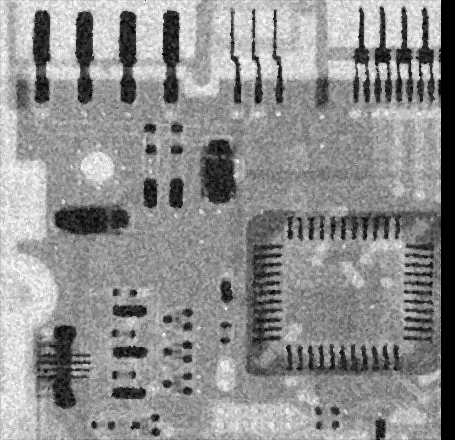
\includegraphics[width=0.9\linewidth]{Q6_1_4_denoised.png}
			\caption{Q6\_1\_4\_denoised}
			\label{Q6_1_4_denoised}
		\end{subfigure}
		\vfill
		\begin{subfigure}[b]{.24\textwidth}
			\centering
			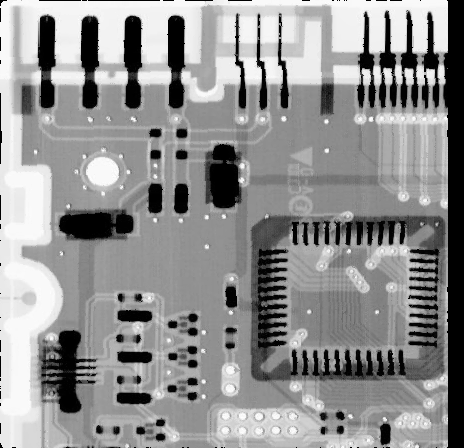
\includegraphics[width=0.9\linewidth]{Q6_1_1_adaptive.png}
			\caption{Q6\_1\_1\_adaptive}
			\label{Q6_1_1_adaptive}
		\end{subfigure}
		\hfill
		\begin{subfigure}[b]{.24\textwidth}
			\centering
			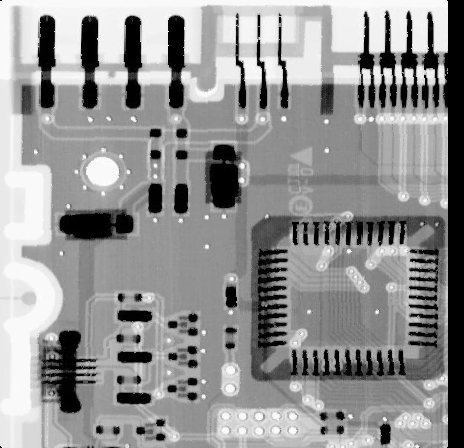
\includegraphics[width=0.9\linewidth]{Q6_1_2_adaptive.png}
			\caption{Q6\_1\_2\_adaptive}
			\label{Q6_1_2_adaptive}
		\end{subfigure}
		\hfill
		\begin{subfigure}[b]{.24\textwidth}
			\centering
			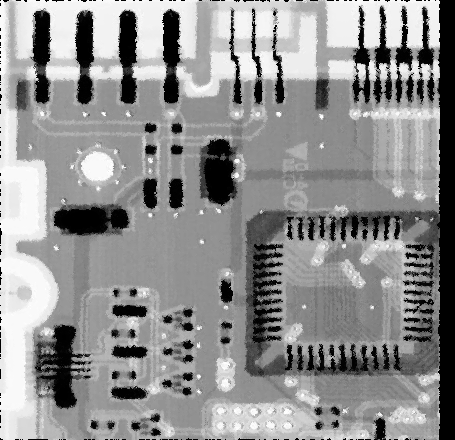
\includegraphics[width=0.9\linewidth]{Q6_1_3_adaptive.png}
			\caption{Q6\_1\_3\_adaptive}
			\label{Q6_1_3_adaptive}
		\end{subfigure}
		\hfill
		\begin{subfigure}[b]{.24\textwidth}
			\centering
			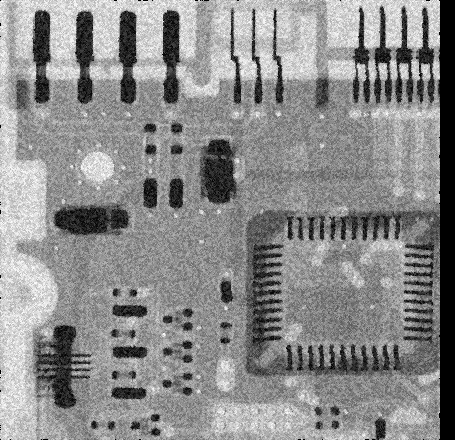
\includegraphics[width=0.9\linewidth]{Q6_1_4_adaptive.png}
			\caption{Q6\_1\_4\_adaptive}
			\label{Q6_1_4_adaptive}
		\end{subfigure}
		\caption{The first line is denoised by smart denosie filter, the second line is denoised by adaptive filter.}
    	\label{Task I, result}	
	\end{figure}

	\subsection*{Discussion}

	From the result we found that, as the intencity of the noise increase, some noise in relatively low frequency domain will remain in the image, that is because the noise have cover most of the information in the image, so some information cannot be restored. And compare two differnet method, we found that the adaptive filter cause less damage to the details.
	

\section*{Task II: Image Restoration}

\begin{problem}
	Image Q6\_2.tif was degraded from an original image due to the atmosphere turbulence given on slide 65 with k = 0.0025. Restore the original image from the input Q6\_2.tif by using full inverse filtering, radially limited inverse filtering and Wiener filtering. Discuss how the parameters, if any, are determined, and the different effects by using the different algorithms.

	\begin{figure}[H]
		\centering
	    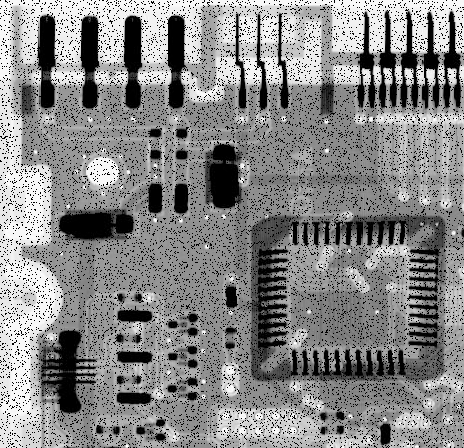
\includegraphics[width=0.3\linewidth]{Q6_1_1.png}
	    \caption{Q6\_1\_1}
	    \label{Q6_1_1}
	\end{figure}
\end{problem}

\subsection*{Analysis}

In this task we will apply three different kinds of inverse filters including full inverse filtering, radially limited inverse filtering and Wiener filtering. Then we will compare the performance of each filter. 

\subsubsection*{full inverse filtering}

The image degrade process can be modeled as image filtering process with degrade filter $$H(u, v)$$ and get result $G(u, v)$, so most directly, the process can be inversed by constructing the inverse filter $$\frac{1}{H(u, v)}$$ Then the inverse filter will be applied to the degraeded image. Here we have $$\widehat{F}(u, v) = \frac{G(u, v)}{H(u, v)}$$ 

In this task we will apply the filters to a image degraded by atmosphere turbulence blur $$H(u, v) = e^{-k(u-M/2)^2+(v-N/2)^2}$$ with k = 0.0025.

\subsubsection*{Radially limited inverse filtering}

The edge of most of the lowpass is close to 0 so when we apply the inverse filter, due to the error in digital computing and image storing, the noise in high frequency will be greatly enhanced, so to avoid the situation, we will add a cutoff filter, here a Butterworth lowpass function of order 10. This provided a sharp (but smooth) transition at the desired radius.

\subsubsection*{Wiener filtering}

Here we discuss an approach that incorporates both the degradation function and statistical characteristics of noise into the restoration process. So that the image degrading during image storing and computing process can be take into consideration.

The filter can be obtained by the expression $$\widehat{F}(u, v)=[\frac{1}{H(u, v)} \frac{|H(u, v)|^2}{|H(u, v)|^2+S_\eta (u, v)/ S_f (u, v)}]G(u, v)$$ However for most of the case we can not get the exact value of $S_\eta (u, v)/ S_f (u, v)$ which represent the signal noise ratio (SNR) of the image, so we will represent it by $K$ so the expression become $$\widehat{F}(u, v)=[\frac{1}{H(u, v)} \frac{|H(u, v)|^2}{|H(u, v)|^2 + K}]G(u, v)$$

\subsection*{Result}

\begin{figure}[H]
	\centering
	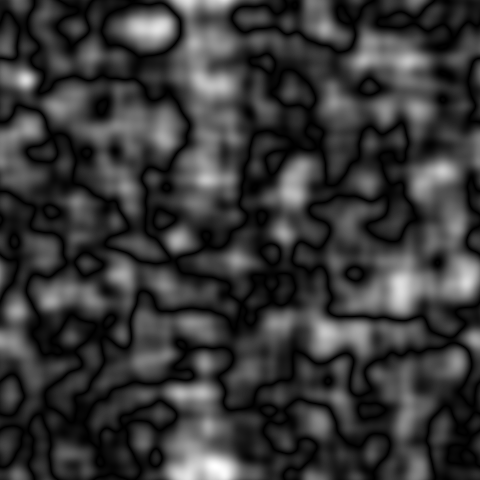
\includegraphics[width=0.3\linewidth]{Q6_2_full_inverse.png}
	\caption{Full inverse filtering}
	\label{Q6_2_full_inverse}
\end{figure}

\begin{figure}[H]
	\centering
	\begin{subfigure}[b]{.3\textwidth}
		\centering
		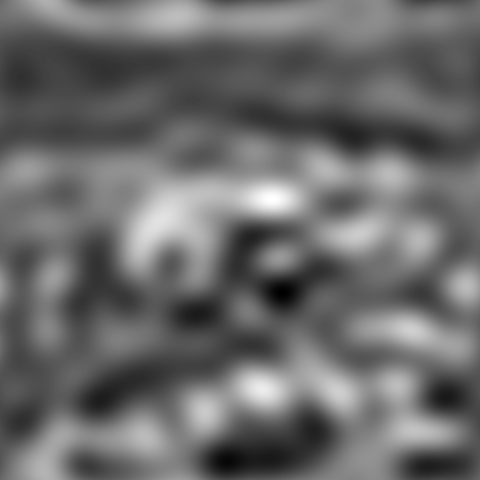
\includegraphics[width=0.9\linewidth]{Q6_2_radially_limited10.png}
		\caption{$\sigma = 10, n = 10$}
		\label{Q6_2_radially_limited10}
	\end{subfigure}
	\hfill
	\begin{subfigure}[b]{.3\textwidth}
		\centering
		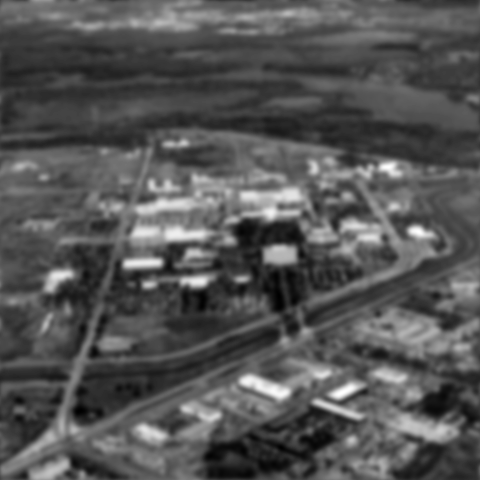
\includegraphics[width=0.9\linewidth]{Q6_2_radially_limited30.png}
		\caption{$\sigma = 30, n = 10$}
		\label{Q6_2_radially_limited30}
	\end{subfigure}
	\hfill
	\begin{subfigure}[b]{.3\textwidth}
		\centering
		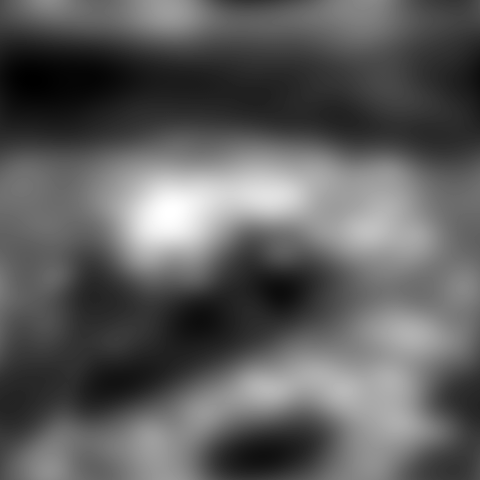
\includegraphics[width=0.9\linewidth]{Q6_2_radially_limited50.png}
		\caption{$\sigma = 50, n = 10$}
		\label{Q6_2_radially_limited50}
	\end{subfigure}
	\vfill
	\begin{subfigure}[b]{.3\textwidth}
		\centering
		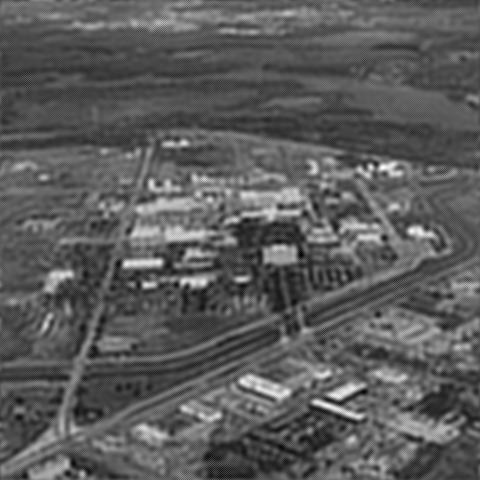
\includegraphics[width=0.9\linewidth]{Q6_2_radially_limited60.png}
		\caption{$\sigma = 60, n = 10$}
		\label{Q6_2_radially_limited60}
	\end{subfigure}
	\hfill
	\begin{subfigure}[b]{.3\textwidth}
		\centering
		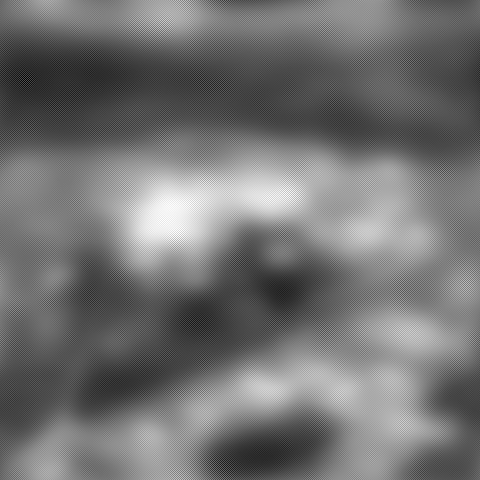
\includegraphics[width=0.9\linewidth]{Q6_2_radially_limited70.png}
		\caption{$\sigma = 70, n = 10$}
		\label{Q6_2_radially_limited70}
	\end{subfigure}
	\hfill
	\begin{subfigure}[b]{.3\textwidth}
		\centering
		
\includegraphics[width=0.9\linewidth]{Q6_2_radially_limited85.png}
		\caption{$\sigma = 85, n = 10$}
		\label{Q6_2_radially_limited85}
	\end{subfigure}
	\caption{Fitered by redially limited inverse filter}
	\label{redially limited inverse filter}	
\end{figure}

\begin{figure}[H]
	\centering
		\begin{subfigure}[b]{.3\textwidth}
			\centering
			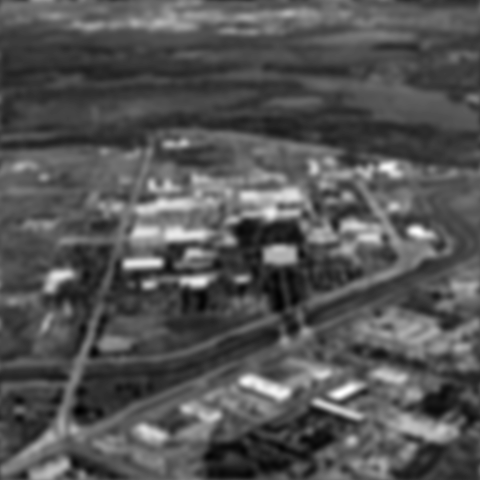
\includegraphics[width=0.9\linewidth]{Q6_2_wiener_50_0.1.png}
			\caption{$\sigma = 50, K = 0.1$}
			\label{Q6_2_wiener_50_0.1}
		\end{subfigure}
		\hfill
		\begin{subfigure}[b]{.3\textwidth}
			\centering
			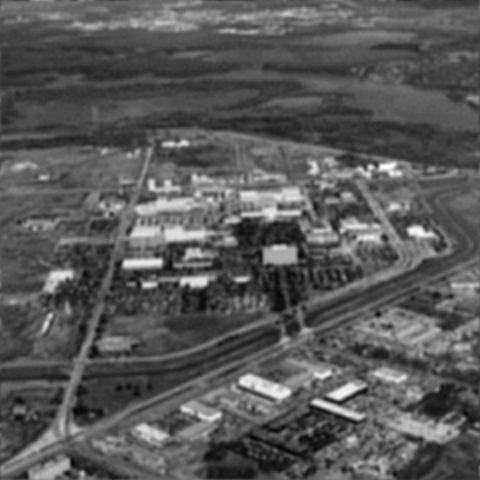
\includegraphics[width=0.9\linewidth]{Q6_2_wiener_50_0.0001.png}
			\caption{$\sigma = 50, K = 10^{-4}$}
			\label{Q6_2_wiener_50_0.001}
		\end{subfigure}
		\hfill
		\begin{subfigure}[b]{.3\textwidth}
			\centering
			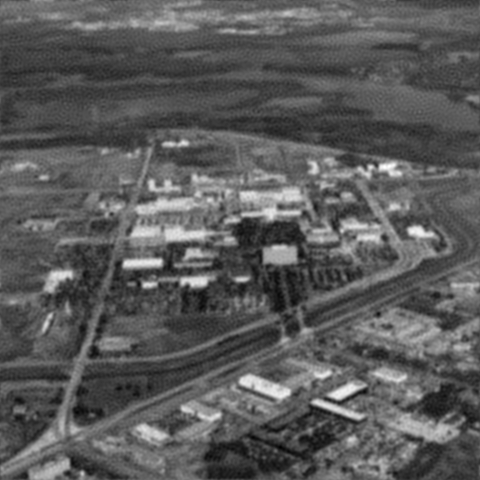
\includegraphics[width=0.9\linewidth]{Q6_2_wiener_50_1e-06.png}
			\caption{$\sigma = 50, K = 10^{-6}$}
			\label{Q6_2_wiener_50_1e-6}
		\end{subfigure}
	\vfill
		\begin{subfigure}[b]{.3\textwidth}
			\centering
			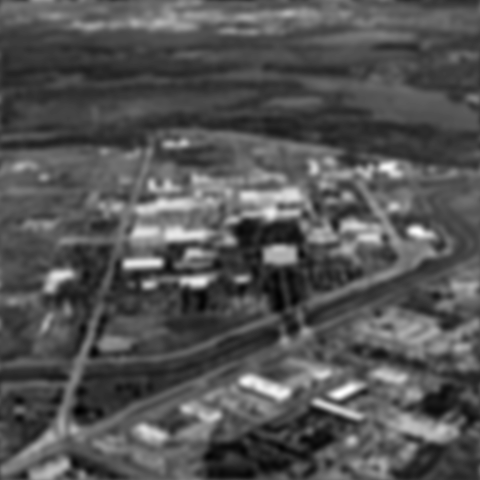
\includegraphics[width=0.9\linewidth]{Q6_2_wiener_60_0.1.png}
			\caption{$\sigma = 60, K = 0.1$}
			\label{Q6_2_wiener_60_0.1}
		\end{subfigure}
		\hfill
		\begin{subfigure}[b]{.3\textwidth}
			\centering
			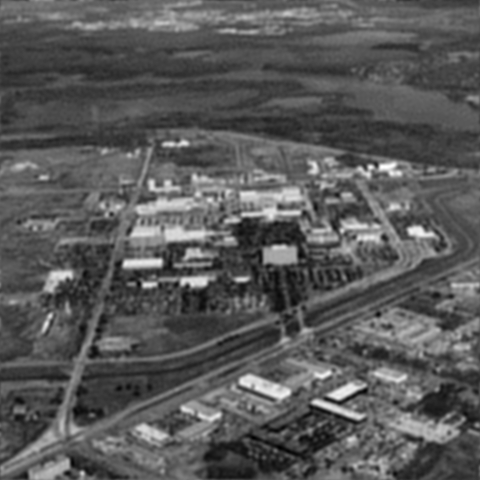
\includegraphics[width=0.9\linewidth]{Q6_2_wiener_60_0.0001.png}
			\caption{$\sigma = 60, K = 10^{-4}$}
			\label{Q6_2_wiener_60_0.001}
		\end{subfigure}
		\hfill
		\begin{subfigure}[b]{.3\textwidth}
			\centering
			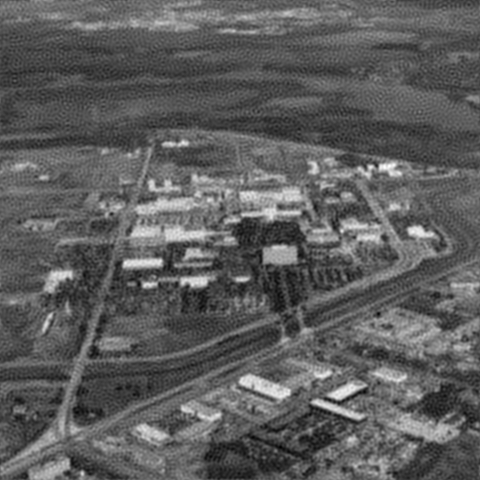
\includegraphics[width=0.9\linewidth]{Q6_2_wiener_60_1e-06.png}
			\caption{$\sigma = 60, K = 10^{-6}$}
			\label{Q6_2_wiener_60_1e-6}
		\end{subfigure}
	\vfill
		\begin{subfigure}[b]{.3\textwidth}
			\centering
			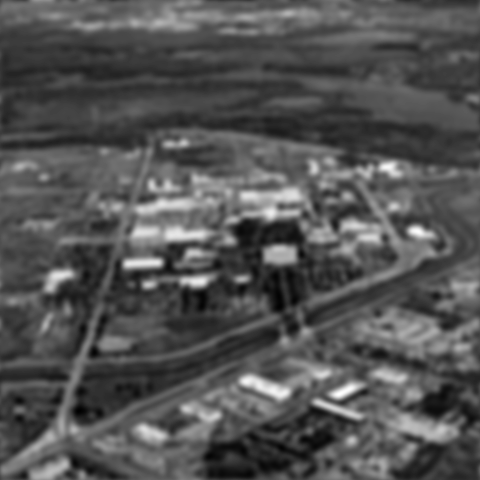
\includegraphics[width=0.9\linewidth]{Q6_2_wiener_70_0.1.png}
			\caption{$\sigma = 70, K = 0.1$}
			\label{Q6_2_wiener_70_0.1}
		\end{subfigure}
		\hfill
		\begin{subfigure}[b]{.3\textwidth}
			\centering
			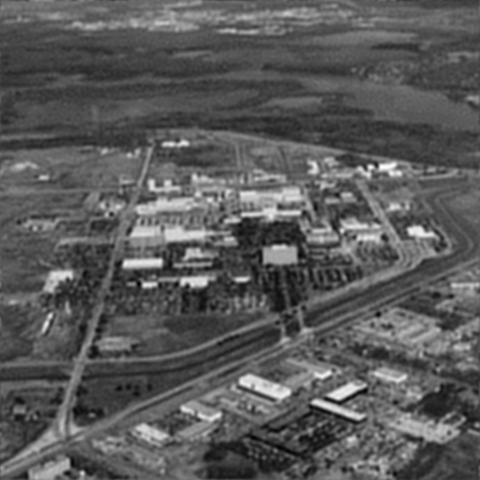
\includegraphics[width=0.9\linewidth]{Q6_2_wiener_70_0.0001.png}
			\caption{$\sigma = 70, K = 10^{-3}$}
			\label{Q6_2_wiener_70_0.001}
		\end{subfigure}
		\hfill
		\begin{subfigure}[b]{.3\textwidth}
			\centering
			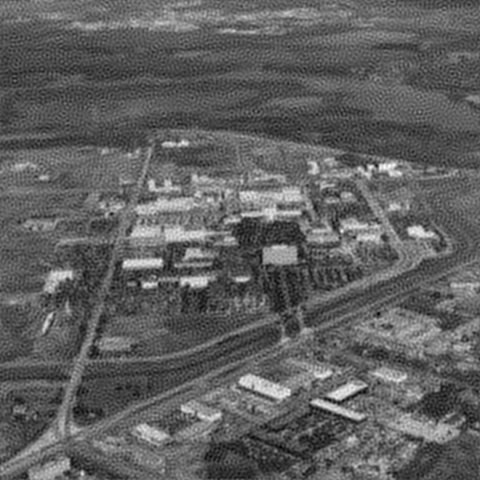
\includegraphics[width=0.9\linewidth]{Q6_2_wiener_70_1e-06.png}
			\caption{$\sigma = 70, K = 10^{-6}$}
			\label{Q6_2_wiener_70_1e-6}
		\end{subfigure}
	\caption{Fitered by wiener filter}
	\label{Fitered by wiener filter}	
\end{figure}

\subsection*{Discussion}

The result shows that full inverse filter is mot capable for most of the case due to the error that may occur that we discussed in the Analysis section. 

Fig \ref{redially limited inverse filter} shows that $\sigma=60$ can be a proper cut off frquency for the filter, when $\sigma$ keeps increase, the high frequency noise will appear again, when $\sigma$ keeps decrease, the details in the image will also be filtered.

Fig \ref{Fitered by wiener filter} shows that $\sigma=60, K = 10^{-6}$can be a proper pair to restore the image by wiener filter, comparing between each image in the image set, when K is decreasing, more details in the image will be restored while the noise increase, that because the detail of the image and noise are similar somehow, so when less detail is filtered, less nise will be filtered. The adjustment of $\sigma$ has been discussed in last paragraph. 

\section*{Task III: Motion Debluring}

\begin{problem}
	Restore the original images from the inputs Q6\_3\_1.tif, Q6\_3\_2.tif and Q6\_3\_3. Explain your observation and the method used.

	\begin{figure}[H]
		\centering
		\begin{subfigure}[b]{.3\textwidth}
			\centering
			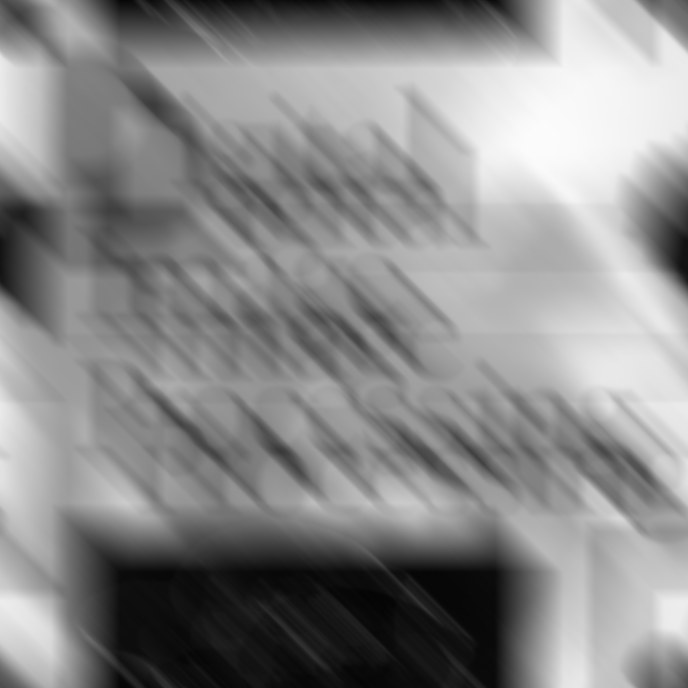
\includegraphics[width=0.9\linewidth]{Q6_3_1.png}
			\caption{Q6\_3\_1}
			\label{Q6_3_1}
		\end{subfigure}
		\hfill
		\begin{subfigure}[b]{.3\textwidth}
			\centering
			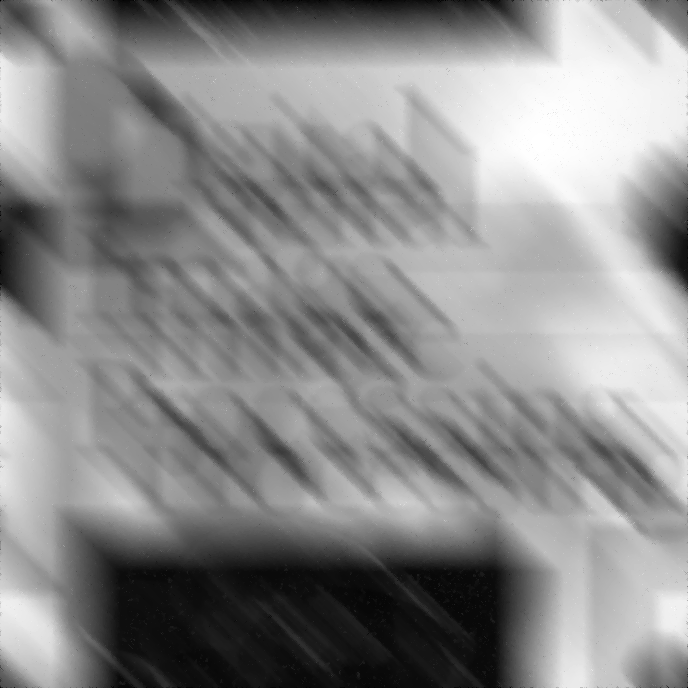
\includegraphics[width=0.9\linewidth]{Q6_3_2.png}
			\caption{Q6\_3\_2}
			\label{Q6_3_2}
		\end{subfigure}
		\hfill
		\begin{subfigure}[b]{.3\textwidth}
			\centering
			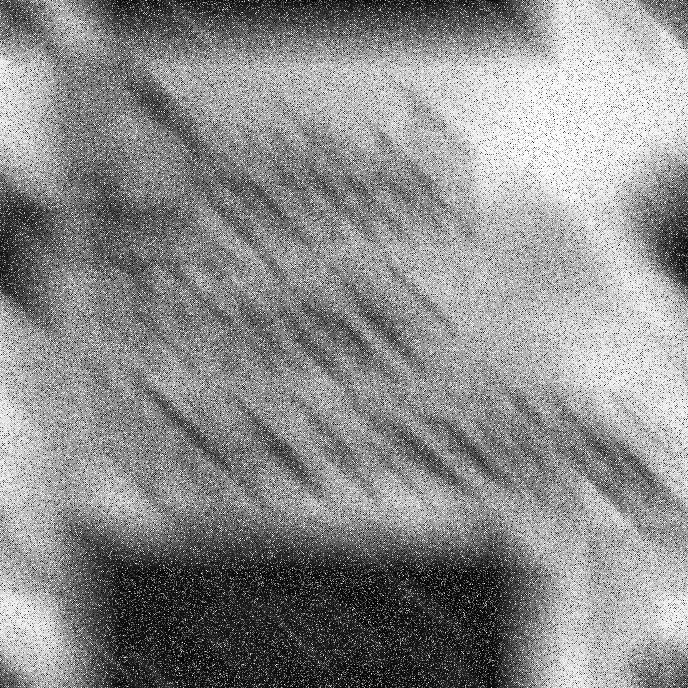
\includegraphics[width=0.9\linewidth]{Q6_3_3.png}
			\caption{Q6\_3\_3}
			\label{Q6_3_3}
		\end{subfigure}
		\caption{Task III, Figures with motion blur}
    	\label{Task III, Figures with motion blur}	
	\end{figure}

\end{problem}

\subsection*{Analysis}

In this task we will reconstruct the image degraded by motion blur and noise. The motion blur can be expressed as filter 

\begin{equation}*
	\begin{aligned}
	H(u, v) &=\int_{0}^{T} e^{-j 2 \pi\left[u x_{0}(t)+v y_{0}(t)\right]} d t \\
	&=\int_{0}^{T} e^{-j 2 \pi[u a+v b] t / T} d t \\
	&=\frac{T}{\pi(u a+v b)} \sin [\pi(u a+v b)] e^{-j \pi(u a+v b)}
	\end{aligned}
\end{equation}

And we will apply radially limited inverse filter and wieber filter to the degreaded image.

\subsection*{Result}

	\begin{figure}[H]
		\centering
		\begin{subfigure}[b]{.24\textwidth}
			\centering
			
\includegraphics[width=0.9\linewidth]{Q6_3_1_radially_limited_1.png}
			\caption{$\sigma=1$}
			\label{Q6_3_1_radially_limited_1}
		\end{subfigure}
		\hfill
		\begin{subfigure}[b]{.24\textwidth}
			\centering
			
\includegraphics[width=0.9\linewidth]{Q6_3_1_radially_limited_10.png}
			\caption{$\sigma=10$}
			\label{Q6_3_1_radially_limited_10}
		\end{subfigure}
		\hfill
		\begin{subfigure}[b]{.24\textwidth}
			\centering
			
\includegraphics[width=0.9\linewidth]{Q6_3_1_radially_limited_50.png}
			\caption{$\sigma=50$}
			\label{Q6_3_1_radially_limited_50}
		\end{subfigure}
		\hfill
		\begin{subfigure}[b]{.24\textwidth}
			\centering
			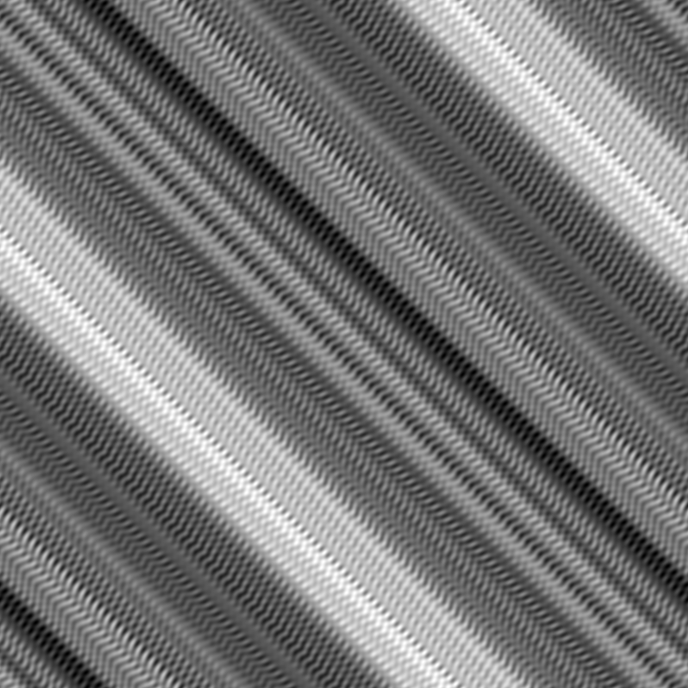
\includegraphics[width=0.9\linewidth]{Q6_3_1_radially_limited_100.png}
			\caption{$\sigma=100$}
			\label{Q6_3_1_radially_limited_100}
		\end{subfigure}
		\caption{Filtered by radially limited inverse filter}
		\label{Motion, radially limited inverse filter}	
	\end{figure}

	\begin{figure}[H]
			\begin{subfigure}[b]{0.3\linewidth}
				\centering
				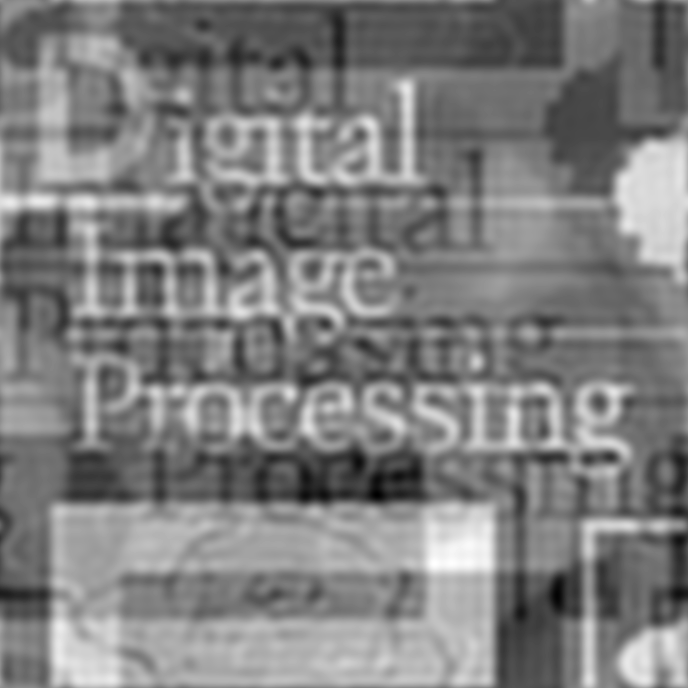
\includegraphics[width=0.9\linewidth]{Q6_3_1_wiener_40_0.1.png}
				\caption{$\sigma = 40, K = 0.1$}
				\label{Q6_3_1_wiener_40_0.1}
			\end{subfigure}
			\hfill
			\begin{subfigure}[b]{0.3\linewidth}
				\centering
				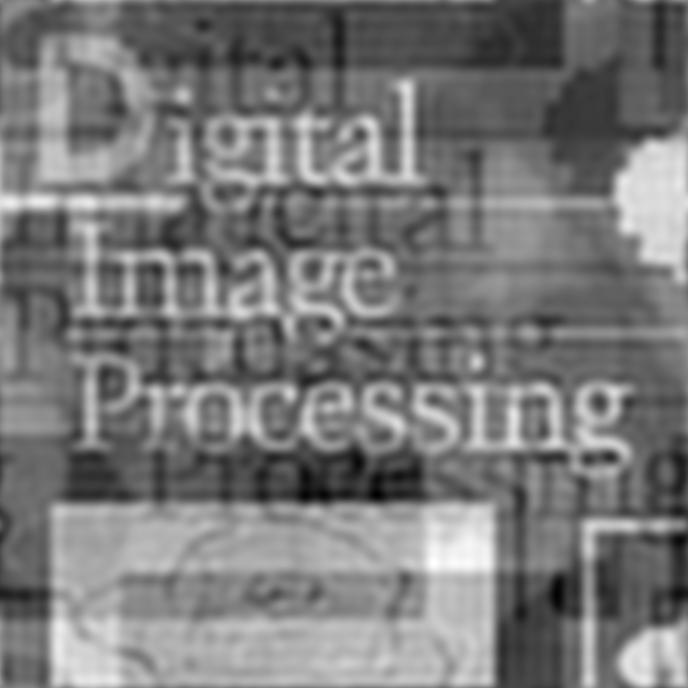
\includegraphics[width=0.9\linewidth]{Q6_3_1_wiener_40_0.0001.png}
				\caption{$\sigma = 40, K = 10^{-4}$}
				\label{Q6_3_1_wiener_40_0.0001}
			\end{subfigure}
			\hfill
			\begin{subfigure}[b]{0.3\linewidth}
				\centering
				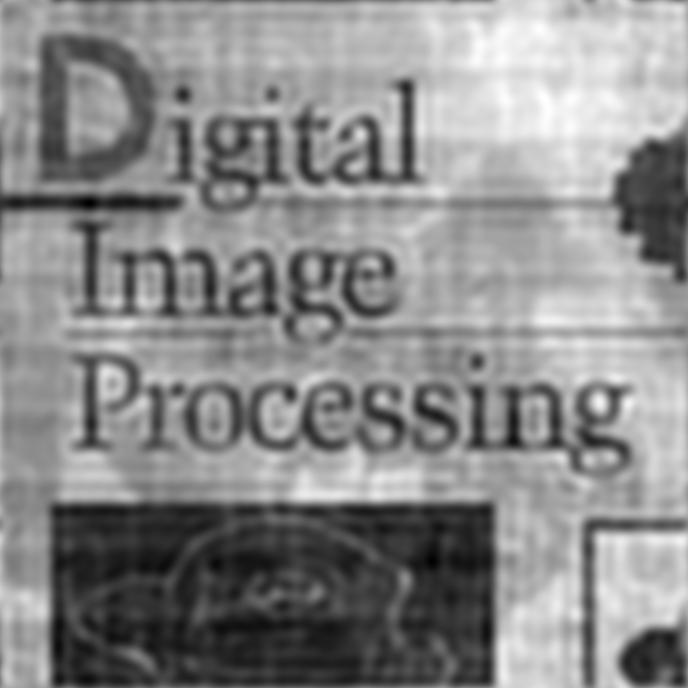
\includegraphics[width=0.9\linewidth]{Q6_3_1_wiener_40_1e-08.png}
				\caption{$\sigma = 40, K = 10^{-8}$}
				\label{Q6_3_1_wiener_40_1e-08}
			\end{subfigure}
		\vfill
			\begin{subfigure}[b]{0.3\linewidth}
				\centering
				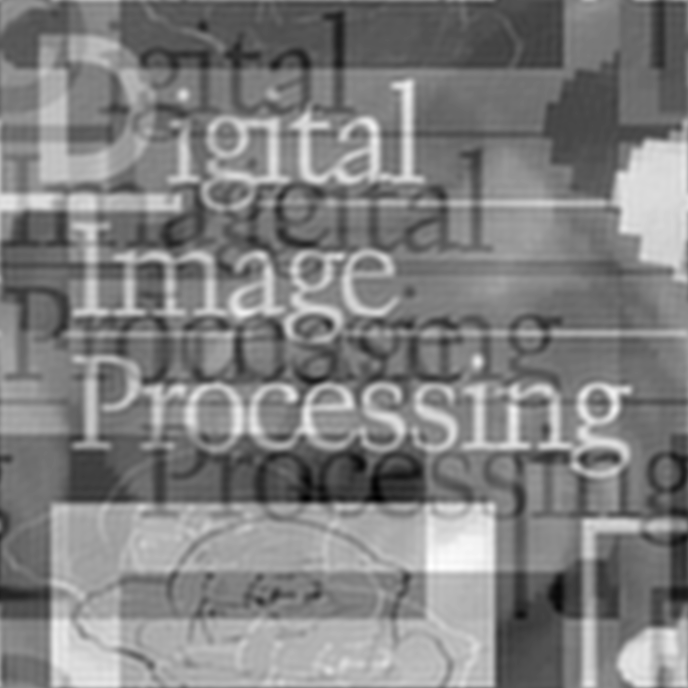
\includegraphics[width=0.9\linewidth]{Q6_3_1_wiener_70_0.1.png}
				\caption{$\sigma = 70, K = 0.1$}
				\label{Q6_3_1_wiener_70_0.1}
			\end{subfigure}
			\hfill
			\begin{subfigure}[b]{0.3\linewidth}
				\centering
				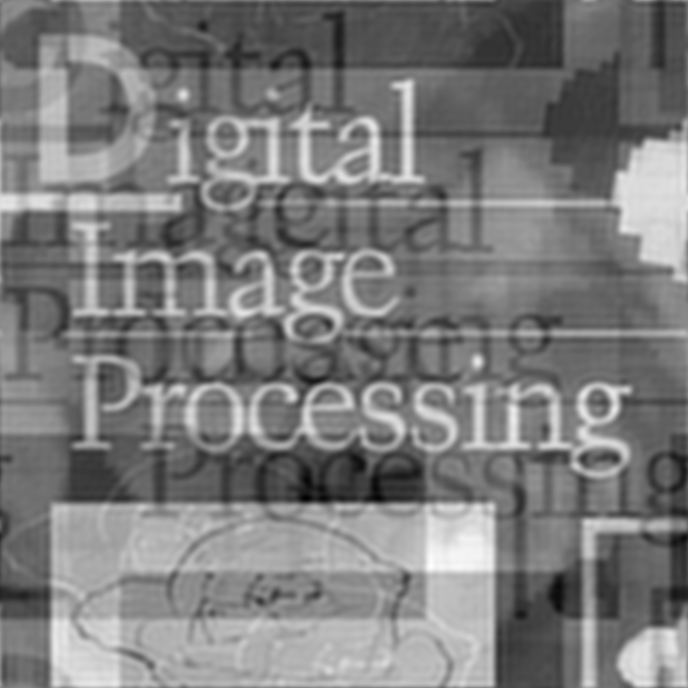
\includegraphics[width=0.9\linewidth]{Q6_3_1_wiener_70_0.0001.png}
				\caption{$\sigma = 70, K = 10^{-4}$}
				\label{Q6_3_1_wiener_70_0.0001}
			\end{subfigure}
			\hfill
			\begin{subfigure}[b]{0.3\linewidth}
				\centering
				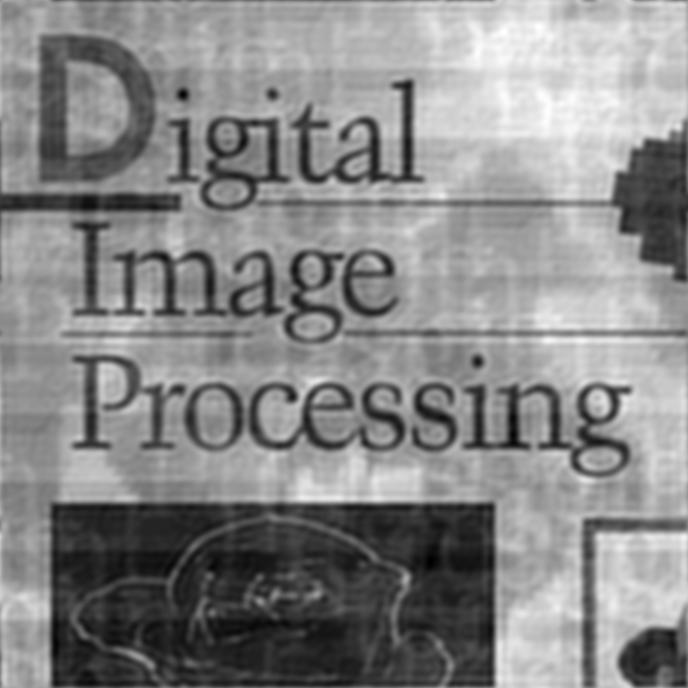
\includegraphics[width=0.9\linewidth]{Q6_3_1_wiener_70_1e-08.png}
				\caption{$\sigma = 70, K = 10^{-8}$}
				\label{Q6_3_1_wiener_70_1e-08}
			\end{subfigure}
		\vfill
			\begin{subfigure}[b]{0.3\linewidth}
				\centering
				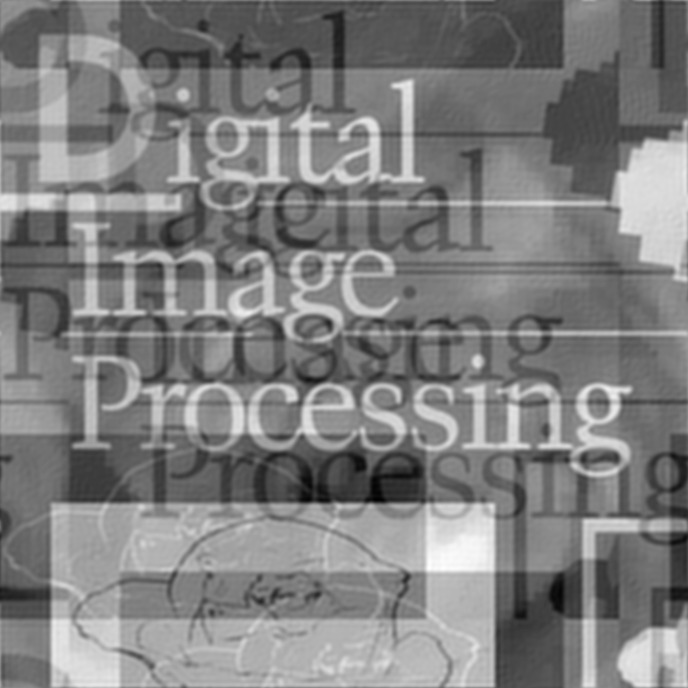
\includegraphics[width=0.9\linewidth]{Q6_3_1_wiener_100_0.1.png}
				\caption{$\sigma = 100, K = 0.1$}
				\label{Q6_3_1_wiener_100_0.1}
			\end{subfigure}
			\hfill
			\begin{subfigure}[b]{0.3\linewidth}
				\centering
				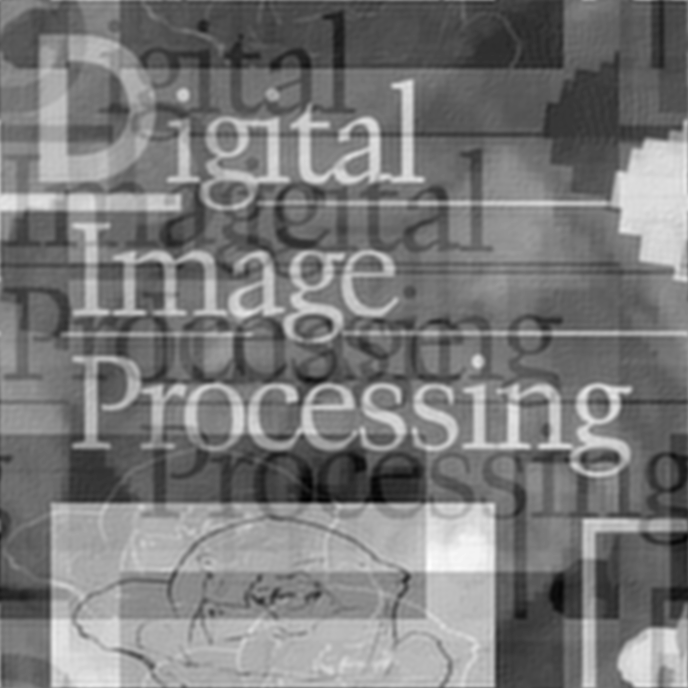
\includegraphics[width=0.9\linewidth]{Q6_3_1_wiener_100_0.0001.png}
				\caption{$\sigma = 100, K = 10^{-4}$}
				\label{Q6_3_1_wiener_100_0.0001.png}
			\end{subfigure}
			\hfill
			\begin{subfigure}[b]{0.3\linewidth}
				\centering
				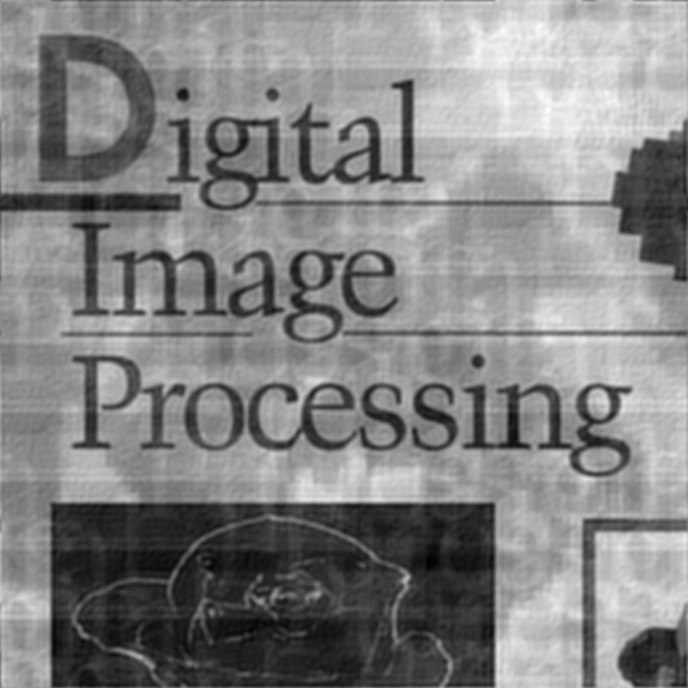
\includegraphics[width=0.9\linewidth]{Q6_3_1_wiener_100_1e-08.png}
				\caption{$\sigma = 100, K = 10^{-8}$}
				\label{Q6_3_1_wiener_100_1e-08}
			\end{subfigure}
		\caption{Fitered by wiener filter}
		\label{Motion wiener filter}
	\end{figure}

	\begin{figure}[H]
		\centering
		\begin{subfigure}[b]{.24\textwidth}
			\centering
			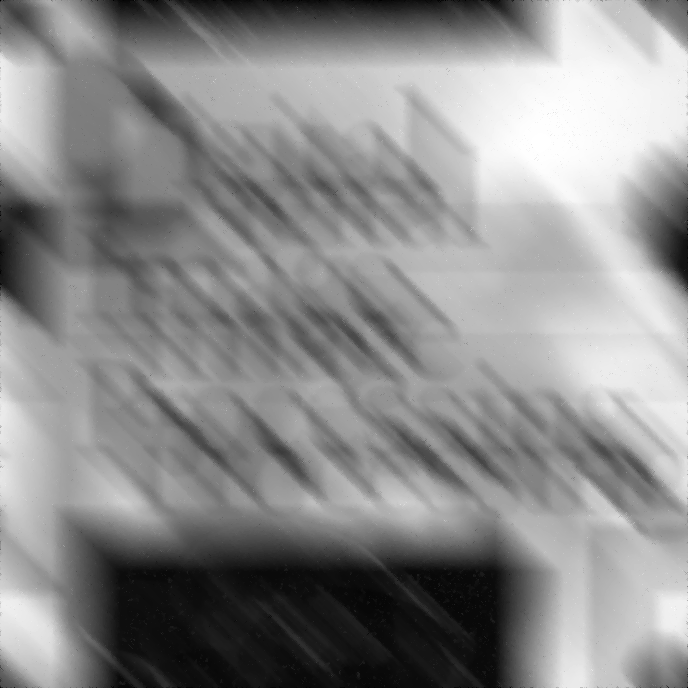
\includegraphics[width=0.9\linewidth]{Q6_3_2.png}
			\caption{Q6\_3\_2}
			\label{Q6_3_2}
		\end{subfigure}
		\hfill
		\begin{subfigure}[b]{.24\textwidth}
			\centering
			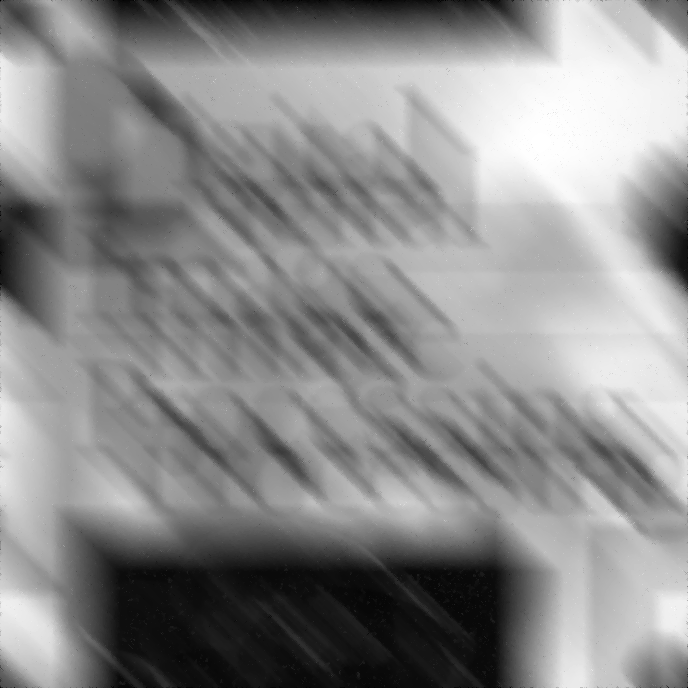
\includegraphics[width=0.9\linewidth]{Q6_3_2_2.png}
			\caption{Q6\_3\_2 denoised}
			\label{Q6_3_2_2}
		\end{subfigure}
		\hfill
		\begin{subfigure}[b]{.24\textwidth}
			\centering
			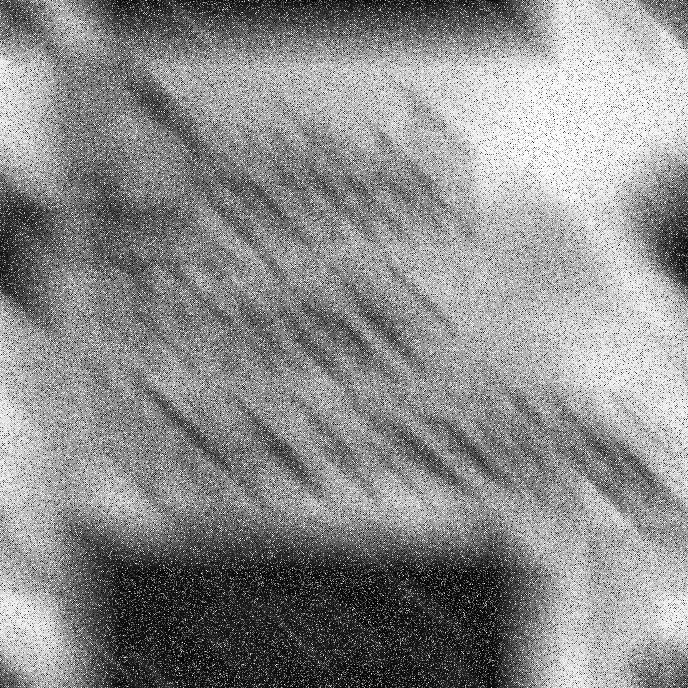
\includegraphics[width=0.9\linewidth]{Q6_3_3.png}
			\caption{Q6\_3\_3}
			\label{Q6_3_3}
		\end{subfigure}
		\hfill
		\begin{subfigure}[b]{.24\textwidth}
			\centering
			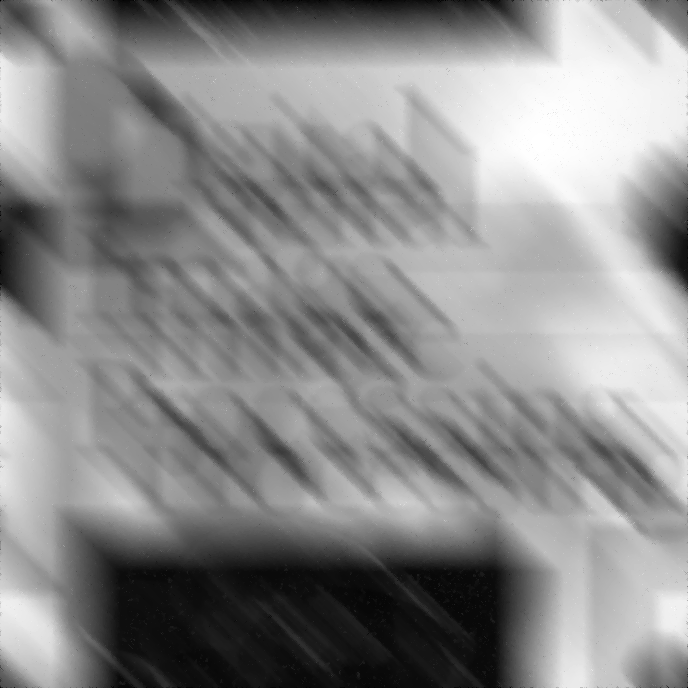
\includegraphics[width=0.9\linewidth]{Q6_3_2_2.png}
			\caption{Q6\_3\_3 denoised}
			\label{Q6_3_2_2}
		\end{subfigure}
		\caption{original image and denoised image}
		\label{original image and denoised image}	
	\end{figure}

	\begin{figure}[H]
		\centering
			\begin{subfigure}[b]{.3\textwidth}
				\centering
				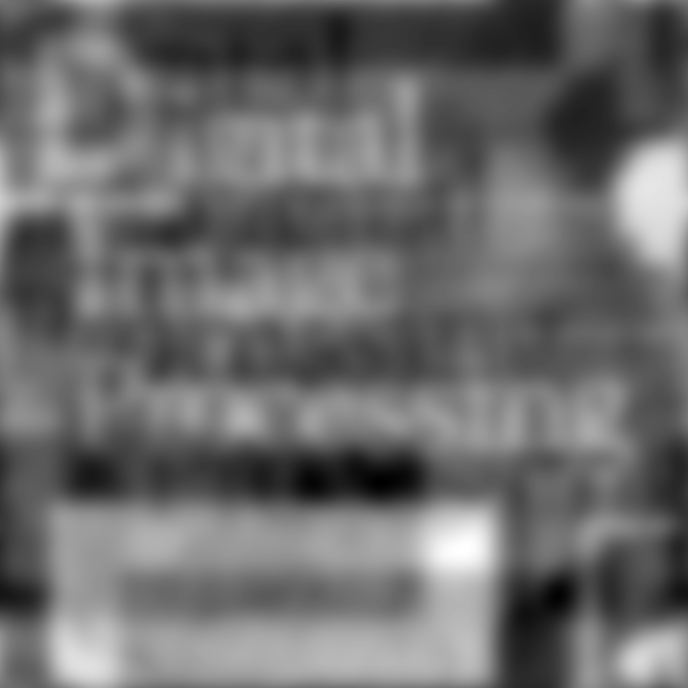
\includegraphics[width=0.9\linewidth]{Q6_3_2_wiener_10_0.25.png}
				\caption{$\sigma=10, K=0.25$}
				\label{Q6_3_2_wiener_10_0.25}
			\end{subfigure}
			\hfill
			\begin{subfigure}[b]{.3\textwidth}
				\centering
				\includegraphics[width=0.9\linewidth]{Q6_3_2_wiener_10_0.0025.png}
				\caption{$\sigma=10, K=0.0025$}
				\label{Q6_3_2_wiener_10_0.0025}
			\end{subfigure}
			\hfill
			\begin{subfigure}[b]{.3\textwidth}
				\centering
				\includegraphics[width=0.9\linewidth]{Q6_3_2_wiener_10_2.5e-05.png}
				\caption{$\sigma=10, K=2.5 \times 10^{-5}$}
				\label{Q6_3_2_wiener_10_2.5e-05}
			\end{subfigure}
		\vfill
			\begin{subfigure}[b]{.3\textwidth}
				\centering
				\includegraphics[width=0.9\linewidth]{Q6_3_2_wiener_50_0.25.png}
				\caption{$\sigma=50, K=0.25$}
				\label{Q6_3_2_wiener_50_0.25}
			\end{subfigure}
			\hfill
			\begin{subfigure}[b]{.3\textwidth}
				\centering
				\includegraphics[width=0.9\linewidth]{Q6_3_2_wiener_50_0.0025.png}
				\caption{$\sigma=50, K=0.0025$}
				\label{Q6_3_2_wiener_50_0.0025}
			\end{subfigure}
			\hfill
			\begin{subfigure}[b]{.3\textwidth}
				\centering
				\includegraphics[width=0.9\linewidth]{Q6_3_2_wiener_50_2.5e-05.png}
				\caption{$\sigma=50, K=2.5 \times 10^{-5}$}
				\label{Q6_3_2_wiener_50_2.5e-05}
			\end{subfigure}
		\vfill
			\begin{subfigure}[b]{.3\textwidth}
				\centering
				\includegraphics[width=0.9\linewidth]{Q6_3_2_wiener_100_0.25.png}
				\caption{$\sigma=100, K=0.25$}
				\label{Q6_3_2_wiener_100_0.25}
			\end{subfigure}
			\hfill
			\begin{subfigure}[b]{.3\textwidth}
				\centering
				\includegraphics[width=0.9\linewidth]{Q6_3_2_wiener_100_0.0025.png}
				\caption{$\sigma=100, K=0.0025$}
				\label{Q6_3_2_wiener_100_0.0025}
			\end{subfigure}
			\hfill
			\begin{subfigure}[b]{.3\textwidth}
				\centering
				\includegraphics[width=0.9\linewidth]{Q6_3_2_wiener_100_2.5e-05.png}
				\caption{$\sigma=100, K=2.5 \times 10^{-5}$}
				\label{Q6_3_2_wiener_100_2.5e-05}
			\end{subfigure}
		\caption{motion deblur of the figure}
		\label{motion deblur of the figure}	
	\end{figure}

\subsection*{Discussion}

Fig \ref{Motion, radially limited inverse filter} indicate that we can't use radially limited inverse filter to restore the image. Here a unit impluse is used to estimate the behavior of the filters

\begin{figure}[H]
	\centering
	\begin{subfigure}[b]{.24\textwidth}
		\centering
		\includegraphics[width=0.9\linewidth]{test_input.png}
		\caption{The unit inpluse \\}
		\label{test_input}
	\end{subfigure}
	\hfill
	\begin{subfigure}[b]{.24\textwidth}
		\centering
		\includegraphics[width=0.9\linewidth]{test_input_burl.png}
		\caption{Motion blur \\}
		\label{test_input_burl}
	\end{subfigure}
	\hfill
	\begin{subfigure}[b]{.24\textwidth}
		\centering
		\includegraphics[width=0.9\linewidth]{test_input_restore_abs.png}
		\caption{inverse filter}
		\label{test_input_restore_abs}
	\end{subfigure}
	\hfill
	\begin{subfigure}[b]{.24\textwidth}
		\centering
		\includegraphics[width=0.9\linewidth]{test_input_restore_winber.png}
		\caption{winber filter}
		\label{test_input_restore_winber}
	\end{subfigure}
	\caption{The behavier of the system to unit impluse}
	\label{unit impluse}	
\end{figure}

After the system is applied to the unit impluse response, we can see a motion blur appeared, then two inverse filters are applied to the degraded image. By inverse filter, the motion blur become more severe, for winber filter, the impluse appear periodicly and their intensity decrease when their distance to the center of the image increase.

However, in previous process, we will save the image and read it again before we apply the inverse filter to it, to save the image, we need to apply \texttt{abs()} function to convert it from complex number to pure real number, so during this process some information is lost. Which create a special kind of noise, then, in further process, the noise is enhanced by the inverse filter. That's why we get useless result in Fig \ref{Motion, radially limited inverse filter}.

Fig \ref{Motion wiener filter} shows the result after restored by wiener filter, here $\sigma = 100, K = 10^{-4}$ is a proper pair to restore the image. Compare between image, if the details of the image is not clear enough, we just increase $\sigma$, if the shadow is to outstanding, we increase the K and if the noise appeared, we increase K.

In addition, the reason of the shadow have been analysised when we apply the system to the unit impluse.

Then we try to apply the filter to image with noise, first we denoise the image by adaptive filter we introduced in section 1, after filtering 3-5 times, we get the filtered image with most of the noise removed, then the wiener filter is applyed to the image. In the result we found that $\sigma =50 K =0.25$, is a proper pair to restore the image, however, there is still a layer of noise in the result, that is because, the denoise process also create lot of noise with differnet motion to the image, so the noise is also enhanced during the filtering.


\section*{Conclusion}

In this lab, we studied adaptive image denoise and image reconstruction method, we found that the adaptive filter is a better method for image denoiseing due to its auto adjusting feature. 

When we use image restoring technic, we have one or multiple parameters to adjust. For example, $\sigma$ in both radially limited inverse filter and wieber filter is used to reduce the high frequency noise, and K in wiener filter can adjust the reduced noise, when we adjust the parameters, one demision of image quality will increase while another decrease, so we need to find a balance between each demision of image quality.

\end{document}
